\chapter{Table recognition implementation}

This chapter gives us an overview of procedures and tools used to create a table recognition software. 

The project is written in C++ and compilable using CMake (tested on MSVC 2017 and GNU 8). We chose CMake for its cross-platform support and its ability to download external dependencies (e.g. Tesseract, Leptonica). 

The implementation is divided into two main parts --- \emph{preprocessing}, which prepares the input images for recognition, and \emph{tabular OCR}, which applies our heuristic algorithm for table recognition. Both parts use the features of the Leptonica library and tabular OCR utilizes the character and textline recognition of the Tesseract engine.

\section{Preprocessing}

The preprocessing part is basically a wrapper around the Leptonica library. Based on the input arguments of our software, the preprocessor calls relevant Leptonica's methods with specified parameters. Not all of the Leptonica's preprocessing features are currently supported in our implementation. However, it is a simple task to add the rest of them. Currently supported methods are the following:

\begin{itemize}
    \item Contrast enhancement
    \item Greyscale conversion
    \item Binarization
    \item Deskewing
\end{itemize}

The initial idea for preprocessing was to provide more complex functions which are included in the OpenCV library. However, this was not the goal of the thesis. Therefore, the preprocessing part stayed very simple and mostly demonstrative and the user is still advised to preprocess the images manually.

\section{Tabular OCR}

After the preprocessing part is done, the preprocessed image is passed to the tabular OCR for table recognition. The individual steps of our heuristic table recognition algorithm are executed in the main \emph{process\_image()} function.

In this section, we analyze this algorithm step-by-step and overview the functions used.

Our algorithm is based on the already mentioned Tesseract symbol and textline recognition and moreover on whitespace detection. Upon detecting whitespaces between individual symbols, we try to heuristically estimate the whitespaces between words and, furthermore, columns, for each textline of the image. Once we have all the textlines separated into columns, we try to merge consecutive lines with similar column layout into a table.  

Following are the individual steps of the algorithm (visualized in~\cref{fig:implemTableRecogniton}):

\begin{enumerate}
\item \emph{Textline initialization}

The whole process begins with the detection of individual characters and their merging into textlines (\cref{fig:implem1}). These textlines are then used during the whole process of the algorithm, and are later searched for words, columns etc.

For the purposes of the character recognition, we use the Tesseract engine. We initialize the Tesseract API without the use of neural networks and obtain both lines and symbols. After this step, we do not use the features of the Tesseract engine anymore, and rely solely on our heuristic functions.

The symbols and lines obtained from Tesseract are represented as simple boxes (with the symbols also containing a textual information). To gain a more detailed information about individual textlines, we therefore iterate over all the lines and symbols and assign symbols into their lines. The result of this function is therefore a list of all textlines containing the information about their individual symbols, like positioning and their actual value in UTF8.

This function runs in $O(m*n^2)$. The initial idea for this implementation was to firstly sort both the symbols and lines by their y coordinates (which is simply $O(\log n)$ and  $O(\log m)$). The assignment of individual symbols into their lines would then be performed by simply iterating symbols and jumping to another line once the current symbol does not fit in the current line, with the iteration therefore having a $O(m*n)$ time complexity. This would present a significant execution time improvement.

However, a problem occurred when iterating symbols. By default, Tesseract's recognition creates a lot of false positives, including noise recognized as dots, white spaces, and, most importantly, horizontal and vertical lines, like footer or header separators, underlinings of words, table borders etc. These false positives disrupt the reading order of the document, which is a factor that this approach relies on.

Although we tried to remove these false positives (for example, removal of empty characters was trivial and required only checking for symbols that contain no textual information), we found no criterion that would suffice all of these obstacles. Therefore, we sacrificed the time complexity in favor of accuracy.

\item \emph{Deletion of unnecessary lines}

As already mentioned, Tesseract's recognition algorithm includes a lot of false positives. In this function, we delete all unnecessary lines (\cref{fig:implem2}), specifically:

\begin{itemize}
\item \emph{Empty lines}

Like horizontal or vertical line segments, borders or other lines that contain no UTF8 symbols are of no use and are therefore deleted from the textline list.

\item \emph{Table textlines}

Table textlines are parts of the image that are bordered by a visible line, which usually represent either a table, form or even a graphics image. Tesseract often recognizes these parts as single textlines. These textlines therefore contain multiple other textlines, and are significantly greater in height. We delete these textlines by simply looking at their height and the font of their symbols.
\end{itemize}

We present both cases in~\cref{fig:deletionOfLines}.

Once this step of the algorithm is done, we are left only with lines that contain symbols and can be a part of the table.

\begin{figure}[t]
\centering
{\sffamily
\begin{tabular}{cc}
Empty lines & Table textline \\
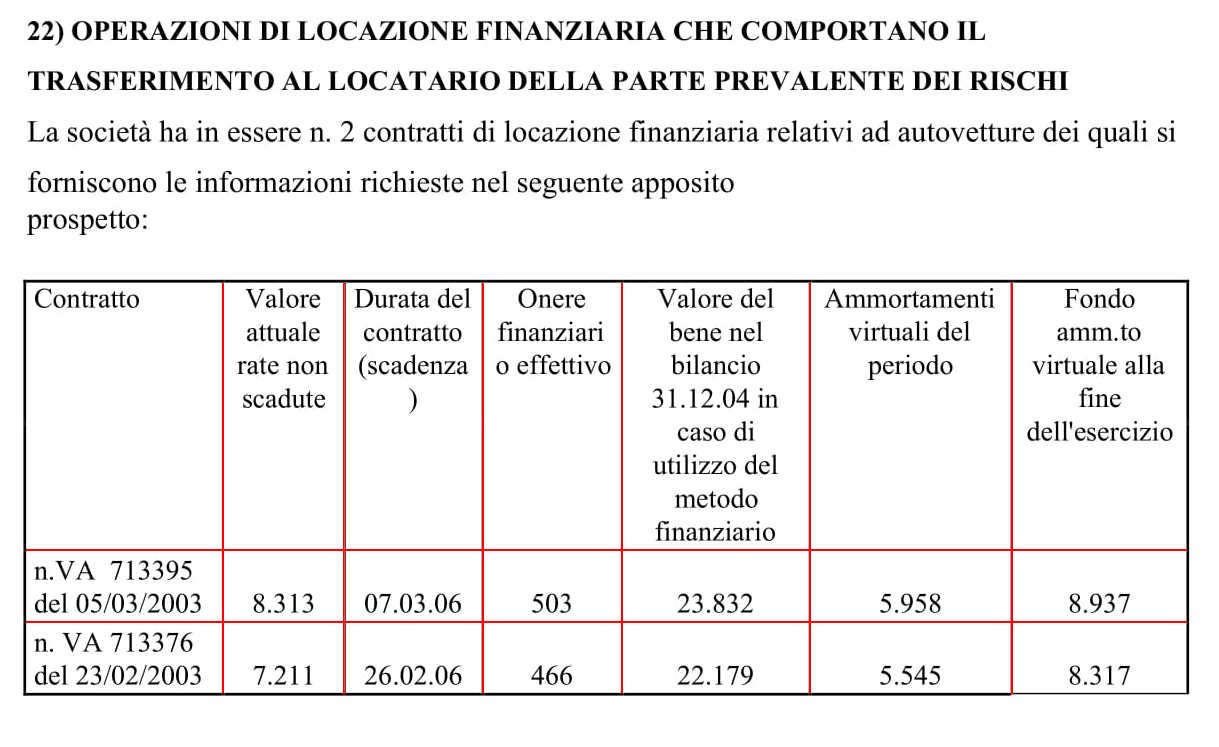
\includegraphics[width=0.4\linewidth]{img/implementation/textlineEmpty.png}
&
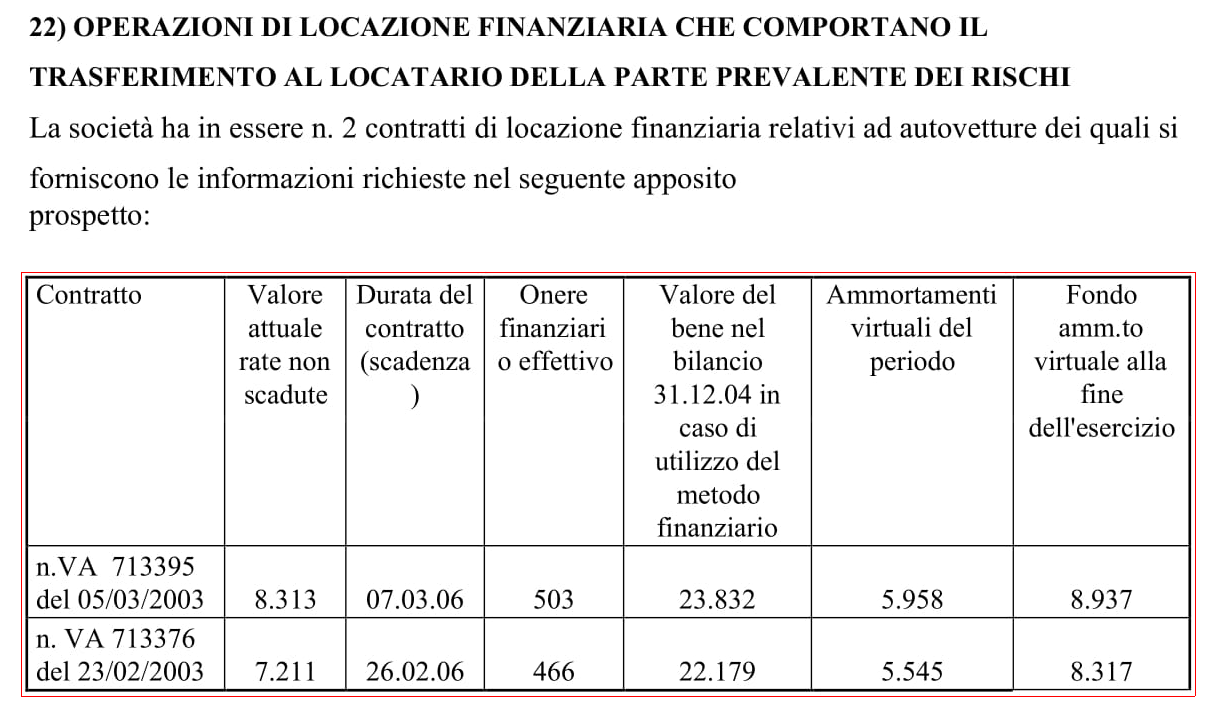
\includegraphics[width=0.4\linewidth]{img/implementation/textlineTable.png}\\
\end{tabular}
}
\caption{Deletion of unnecessary lines}
\label{fig:deletionOfLines}
\end{figure}

\item \emph{Column detection} \label{columnDetection}

Upon obtaining individual textlines, we try to determine their segmentation into columns by analyzing the symbols they contain. This is done for each line individually. Firstly, we merge symbols into words. After that, we merge words into columns (\cref{fig:implem3}). Although we could simply just merge symbols into columns and ignore the whole processing of words, this would leave us with no information about spaces between individual words and would therefore lead to merging of text.

We start this process by obtaining all the spaces between individual symbols and sorting them by size. For human perception, upon seeing this list, to determine the whitespace between individual words and columns is mostly an intuitive and easy task. Following are three lists of spaces. We present the visualized merge of our algorithm according to them in~\cref{fig:symbolMerging}.
and a visualized merge of our algorithm according to them:

\texttt{1 1 2 2 2 3 3 3 3 3 3 3 3 3 3 3 3 4 4 4 4 5 15 15 16 16 18 18 227 235;}

\texttt{2 2 2 2 2 2 2 2 2 3 3 3 3 3 3 3 3 3 3 3 3 4 4 4 4 4 4 4 5 5 6 15 15 16 17 165 235;}

\texttt{1 1 1 2 2 2 3 3 3 3 3 3 3 3 3 3 3 4 4 4 4 4 4 4 4 5 5 15 15 15 17 17 17 18 134 235;}

\begin{figure}[t]
\centering
{\sffamily
\begin{tabular}{c}
The original image \\
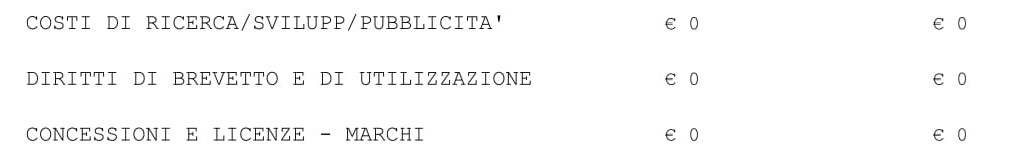
\includegraphics[width=0.8\linewidth]{img/implementation/mergedOrig.jpg}\\
Merged into words \\
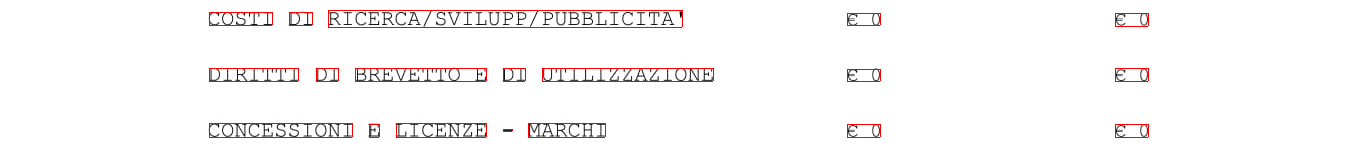
\includegraphics[width=0.8\linewidth]{img/implementation/mergedWords.png}\\
Merged into columns \\
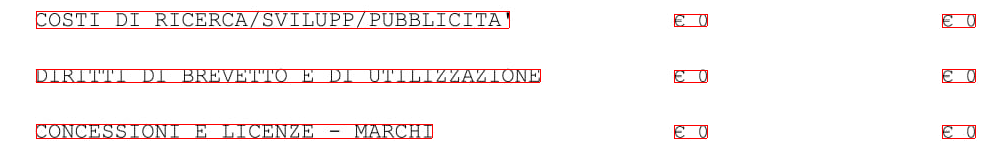
\includegraphics[width=0.8\linewidth]{img/implementation/mergedCols.png}\\
\end{tabular}
}
\caption{The process of merging symbols of a textline}
\label{fig:symbolMerging}
\end{figure}

It is quite obvious that the word whitespace will therefore be around 5-6 in all cases and column whitespace 227, 165 and 134 respectively. In our implementation, we determine these whitespaces by iterating over all the symbol spaces. Once we find two subsequent spaces that have "great difference between their values", we assume the greater one to be the whitespace of either words, columns or both.

So how do we determine whether the difference is too great? For both word and column whitespaces, we calculate a so-called \emph{multiplicator factor} and use it according to the next code snippet that is used for the determination of the word whitespace:

\begin{code}
for (it; it != all_spaces.end() - 1; it++)
{
  // get multiplication factor of current space
  double multi_factor = get_multi_factor_words(*it, constant);
  if (*std::next(it) >= multi_factor * *it)
  {
    // found the word whitespace at *std::next(it)
    // code to execute once the whitespace is found
  }
}
\end{code}

From the results of the detection of spaces between individual symbols, we observed that the greater the current space is, the less the multiplication factor should be. Based on this, we have tried many different values and curves for the determination of the multiplication factor. First observations from these attempts led to the estimation that the best curve to use would be logarithmic. However, the current implementation seemed to worked well enough and was therefore left as it is.

The determination of the column whitespace was based on a similar idea with slightly altered parameters.

Upon determining the column and word whitespaces, we then merge symbols by these whitespaces into words and columns respectively.

The determination of whitespaces was probably the most difficult part of the algorithm. There have been multiple different ideas for the implementation. The one that has been preferred most of the time was the idea of separating textlines according to their \emph{font sizes}. The ones with similar fonts were assigned to the same \emph{font category}, and the whitespace was then determined for the whole category. The word whitespace recognition worked slightly better with this approach. However, the determination of columns had a higher chance of failure, as the sizes of column spaces differed greatly and the algorithm encountered problems when finding the point where word spaces ended and column spaces started. Therefore, the current simpler approach was chosen.

Another initial idea was to simply determine the size of the column space by a constant, e.g. word\_whitespace*constant = column\_whitespace. Surprisingly, the results of this approach were comparable to those of the current implementation. However, it was deemed to fail when it came to small fonts or full-page tables, and had no room for improvement in contrast with the current approach.

\item \emph{Table creation}

Once we have the information about columns for each textline, we can start searching for tables. The table detection algorithm is performed by a simple $O(n)$ algorithm by iterating the textlines from top to bottom and merging two consecutive textlines with a similar column layout into a table.

The determination of a similar column layout is performed by~\cref{alg:tableMerge}. \xxx{?}

Merge of the textlines is done by merging columns that have been detected to overlap, and adding other columns with no such attribute. In a typical $m{\times}n$ table, every column should overlap with the one underneath it, which is also mostly the case when running this algorithm.

Once we have at least two merged textlines, we use this new merged line as a current textline. Therefore, when creating a table, we append new lines to the already merged ones. At the end of this algorithm, our current table is therefore represented as a textline with the information about its columns (and a list of textlines that are in the current table).

\begin{algorithm}[t]
\caption{Are textlines in same table}
\label{alg:tableMerge}
\begin{algorithmic}
\State $iter\_first$ represents the current place we are when iterating over columns of first line
\State $iter\_second$ represents the current place we are when iterating over columns of second line
\While{true}
\If {either $iter\_first$ or $iter\_second$ is at the end of their line}
\If {at least one pair of columns was found that should be merged}
\State \emph{merge()}
\EndIf
\EndIf
\If {current\_columns\_overlap() } \Comment{a function that checks whether the bounding boxes of the two columns overlap in the x axis}
\If {found columns do not overlap with other existing columns in the x axis}
\State save the position of overlapping columns for future mergeing
\EndIf
\Else 
\State increase either $iter\_first$ or $iter\_second$ depending on which is poiting to the box that has a lower x-axis
\State continue
\EndIf
\State $iter\_first \gets iter\_first+1$
\State $iter\_second \gets iter\_second+1$
\EndWhile
\end{algorithmic}
\end{algorithm}

\item \emph{Output creation}

What we focus on when creating an output are table cells. We create them by simply overlaying rows and columns and saving their common areas as cells. The problem arises with the existence of multi-line rows, that is, rows that often span over multiple textlines. In our implementation, a simple constant-based algorithm is added to recognize at least some of them and therefore merge multiple textlines into one row.

Once we obtain the cells, the only thing left is to create a user-friendly representation of the recognized data. Here, the user has two options according to the parameter he sets in the command line environment. 

The first option is a simple image output. Recognized cells are therefore bordered by colored boxes (\cref{fig:implem4}) in the original input image and saved in a PNG file.

The other option is a json structure of the recognized cells, which also contains text within each cell. The json has the following structure:

\lstset{
    string=[s]{"}{"},
    stringstyle=\color{blue},
    comment=[l]{:},
    commentstyle=\color{black},
}
\begin{lstlisting}
{"all_tables": {
  "cols": number of columns,
  "rows": number of rows,
  "table_repres": {
    "h": height of table,
    "w": width of table,
    "x": the x-coordinate where the table starts
    "y": the y-coordinate where the table starts
  }
  "cells": [
        {
        "box": {
           "h": height of current cell,
           "w": width of current cell,
           "x": the x-coordinate where the cell starts,
           "y": they y-coordinate where the cells starts,
        },
        "cols_no": in which column of the table the cell is,
        "rows_no": in which row of the table the cell is,
        "text": the UTF8 text displayed in the cell
        },
        ...
        other cells
    ]
  }
  ...
  other tables
}
\end{lstlisting}

By default, both output options are selected and therefore two files are saved in the newly created \emph{results} directory inside the build directory.

\end{enumerate}

We present the whole process of the implementation, starting from the moment command line arguments are being processed to the last processed image in~\cref{fig:programFlow}.

\begin{figure}[t]
\begin{subfigure}{0.45\textwidth}
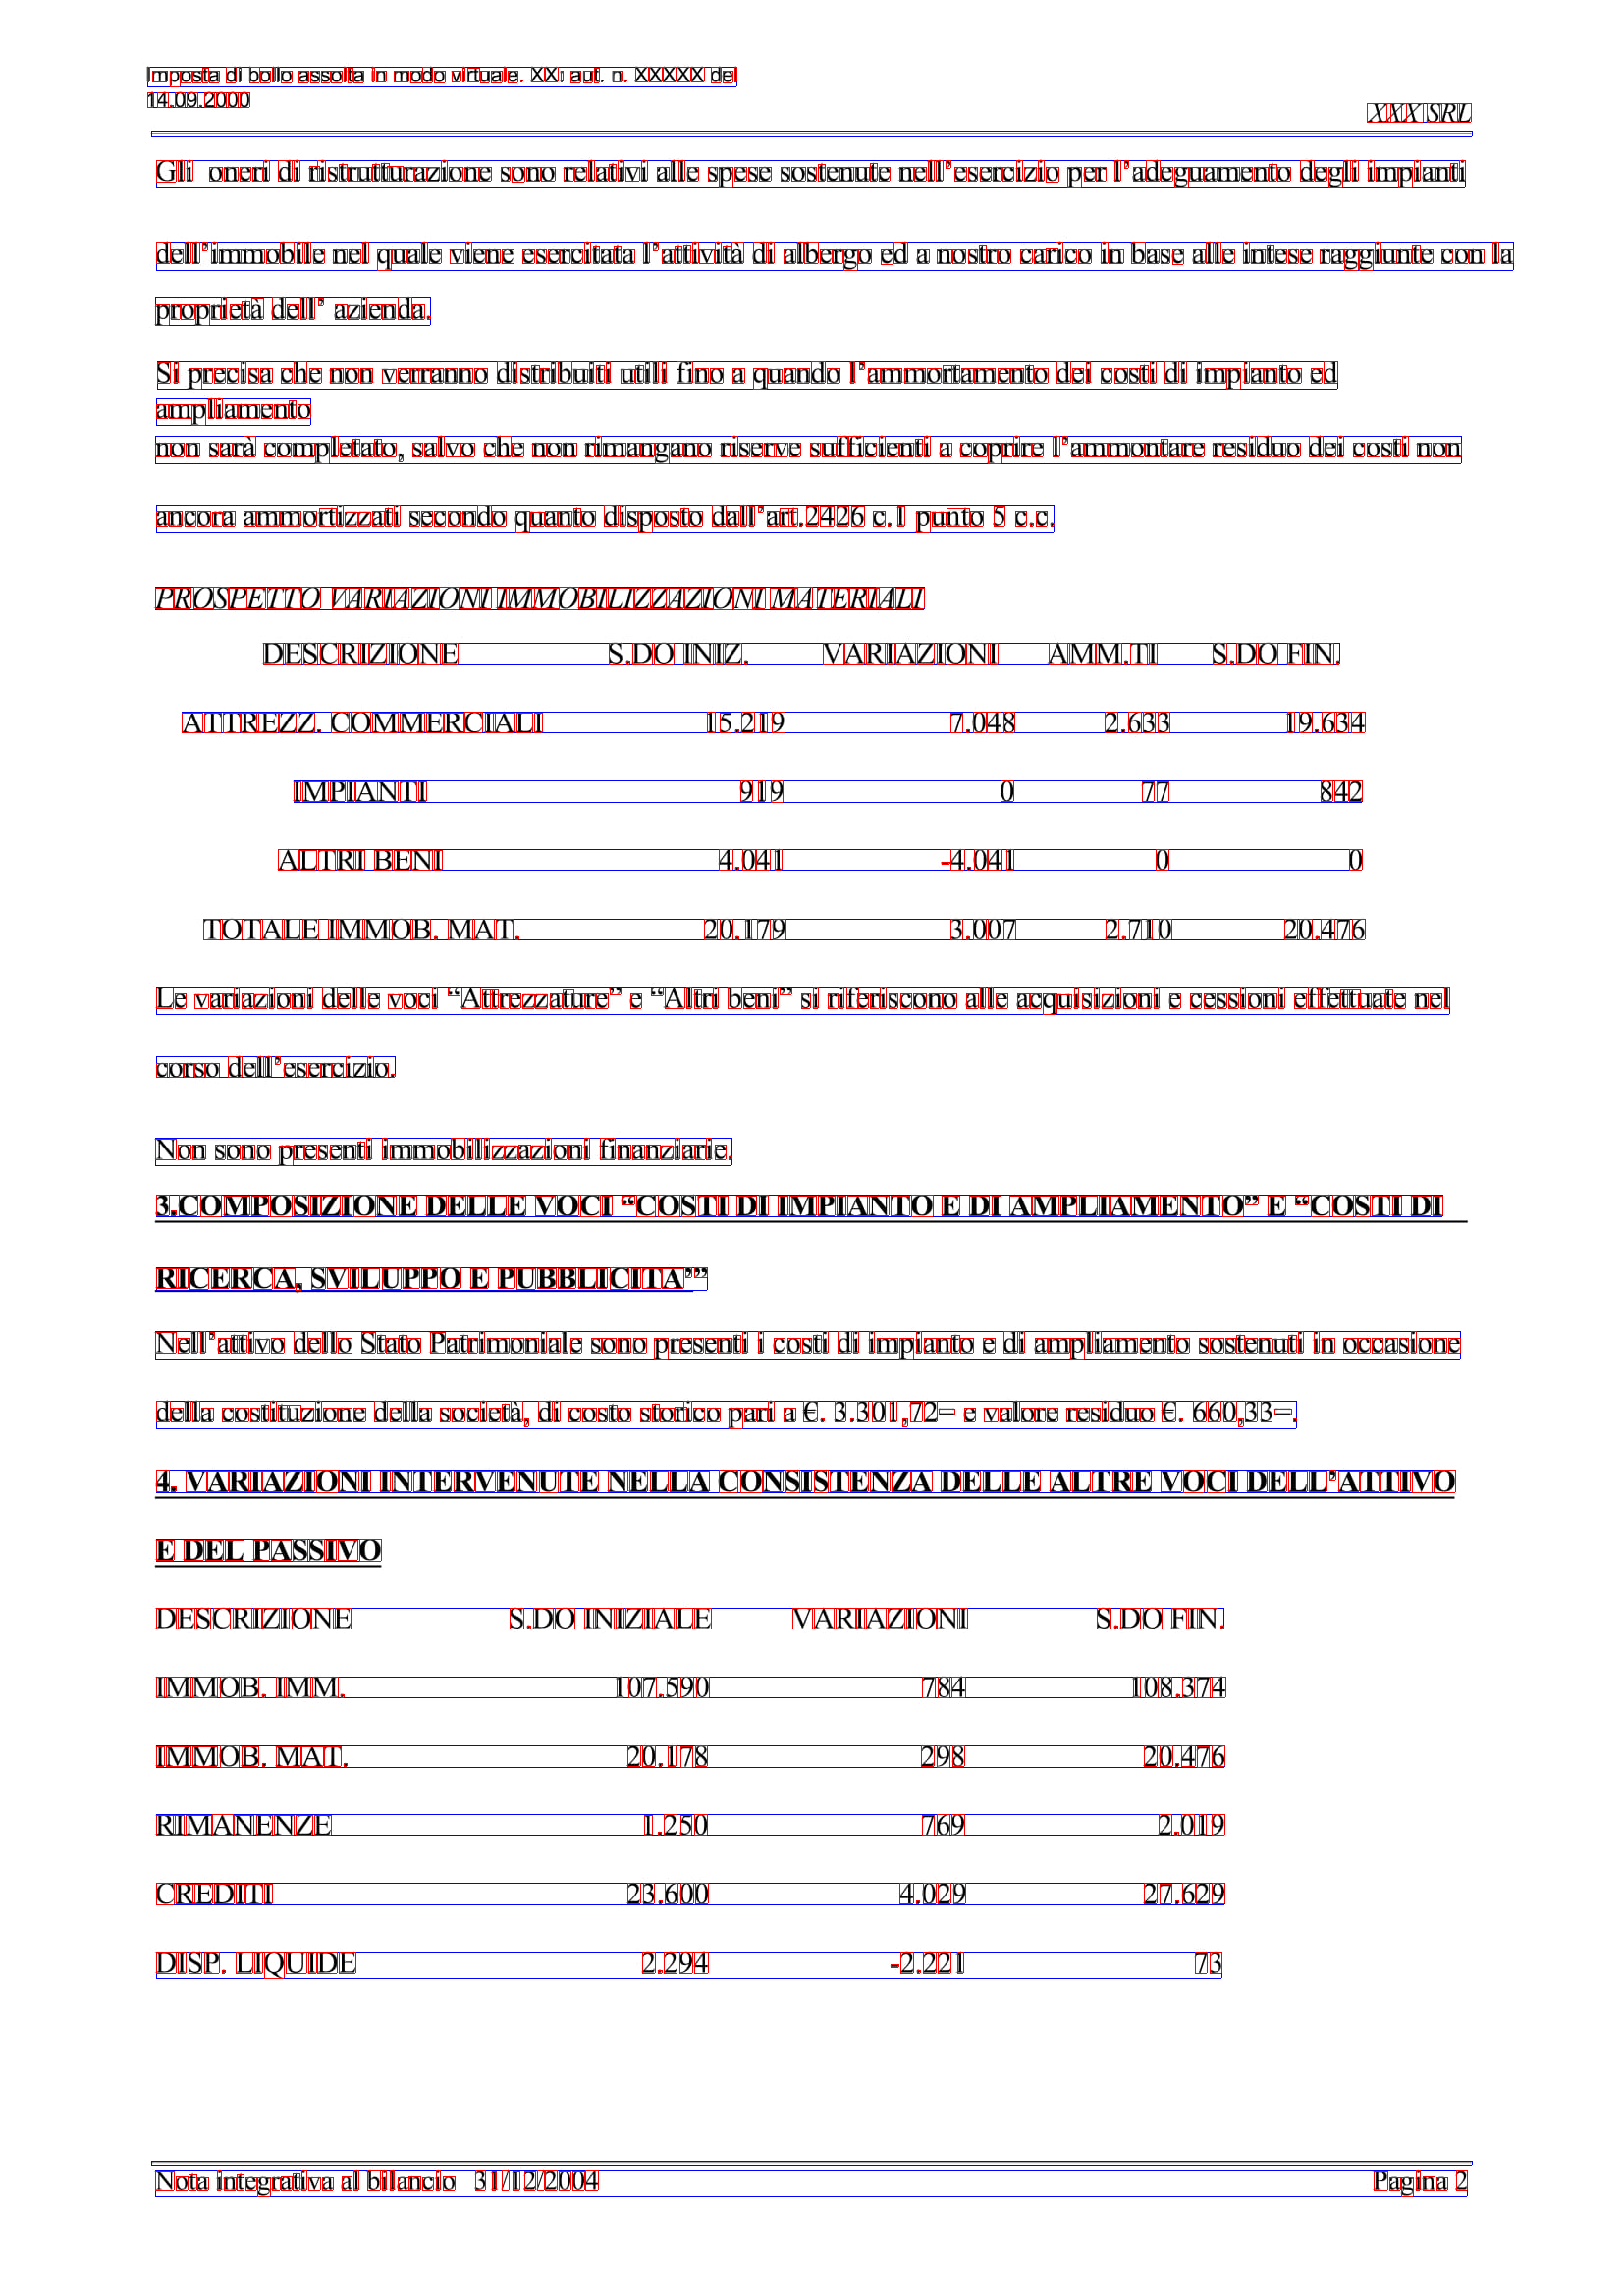
\includegraphics[width=\linewidth]{img/implementation/implem1.png}
\caption{Individual textlines (blue) and their symbols (red)}
\label{fig:implem1}
\end{subfigure}
\qquad
\begin{subfigure}{0.45\textwidth}
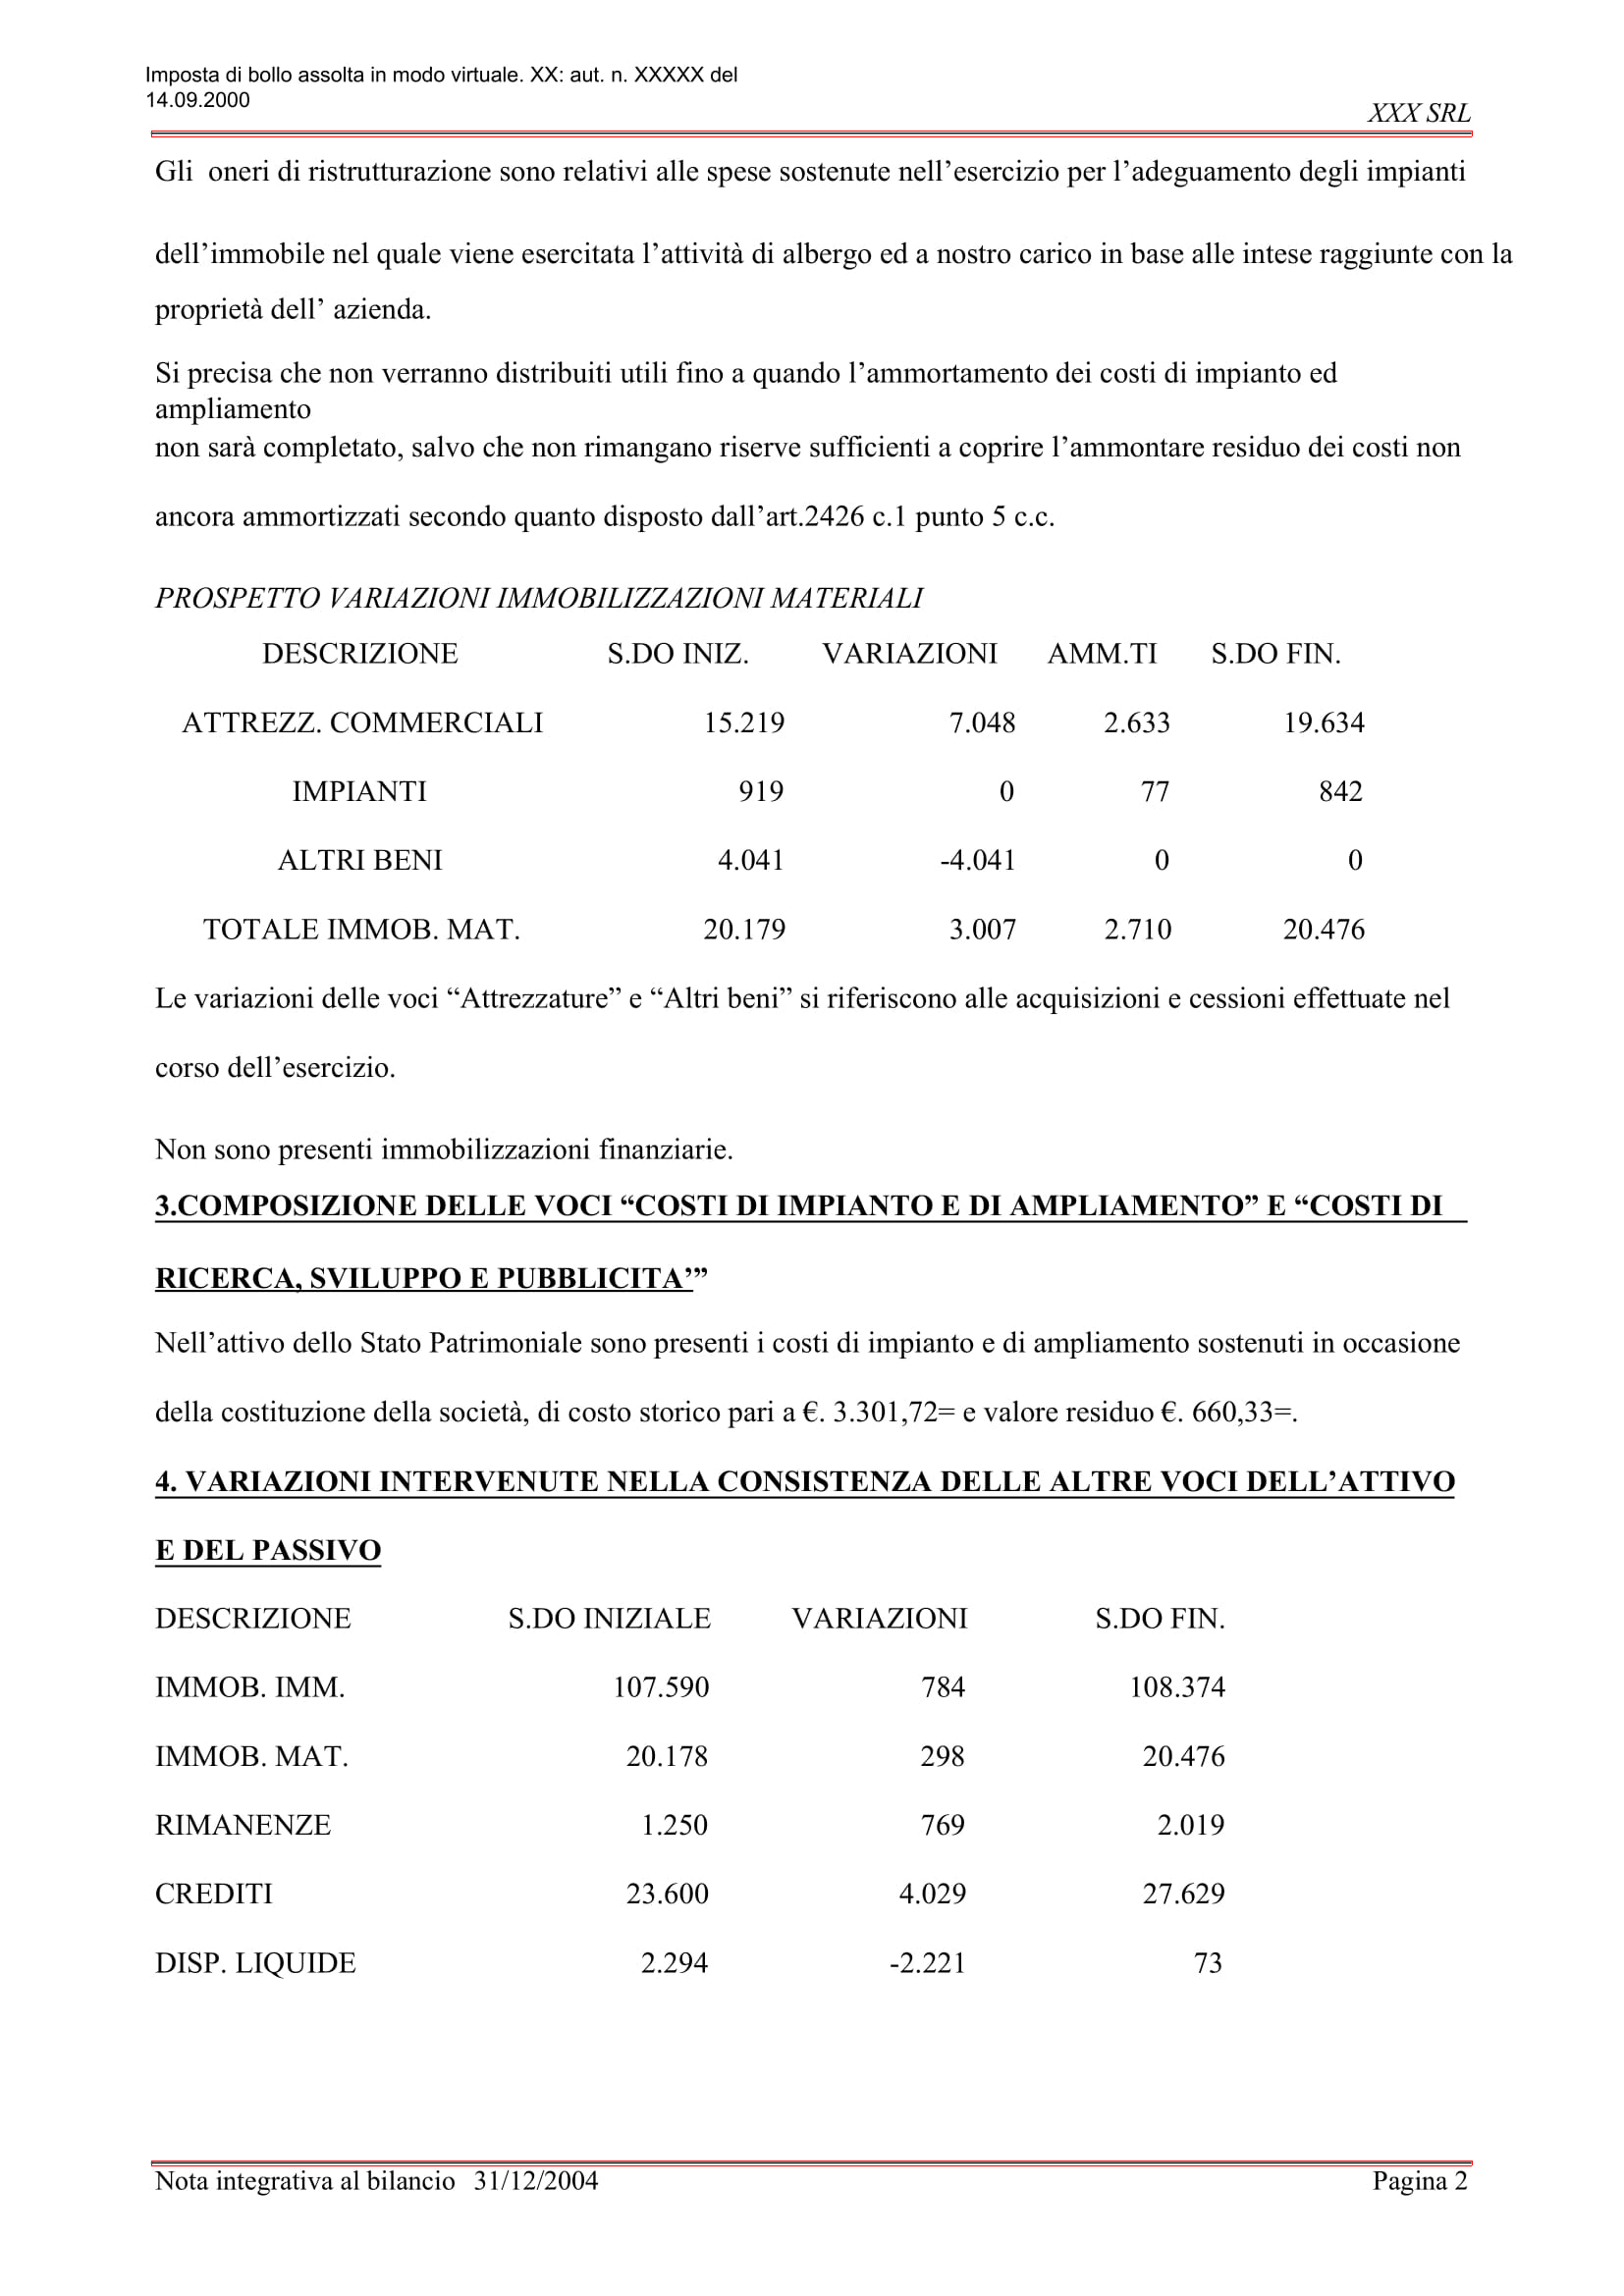
\includegraphics[width=\linewidth]{img/implementation/implem2.png}
\caption{Unnecessary lines}
\label{fig:implem2}
\end{subfigure}
\begin{subfigure}{0.45\textwidth}
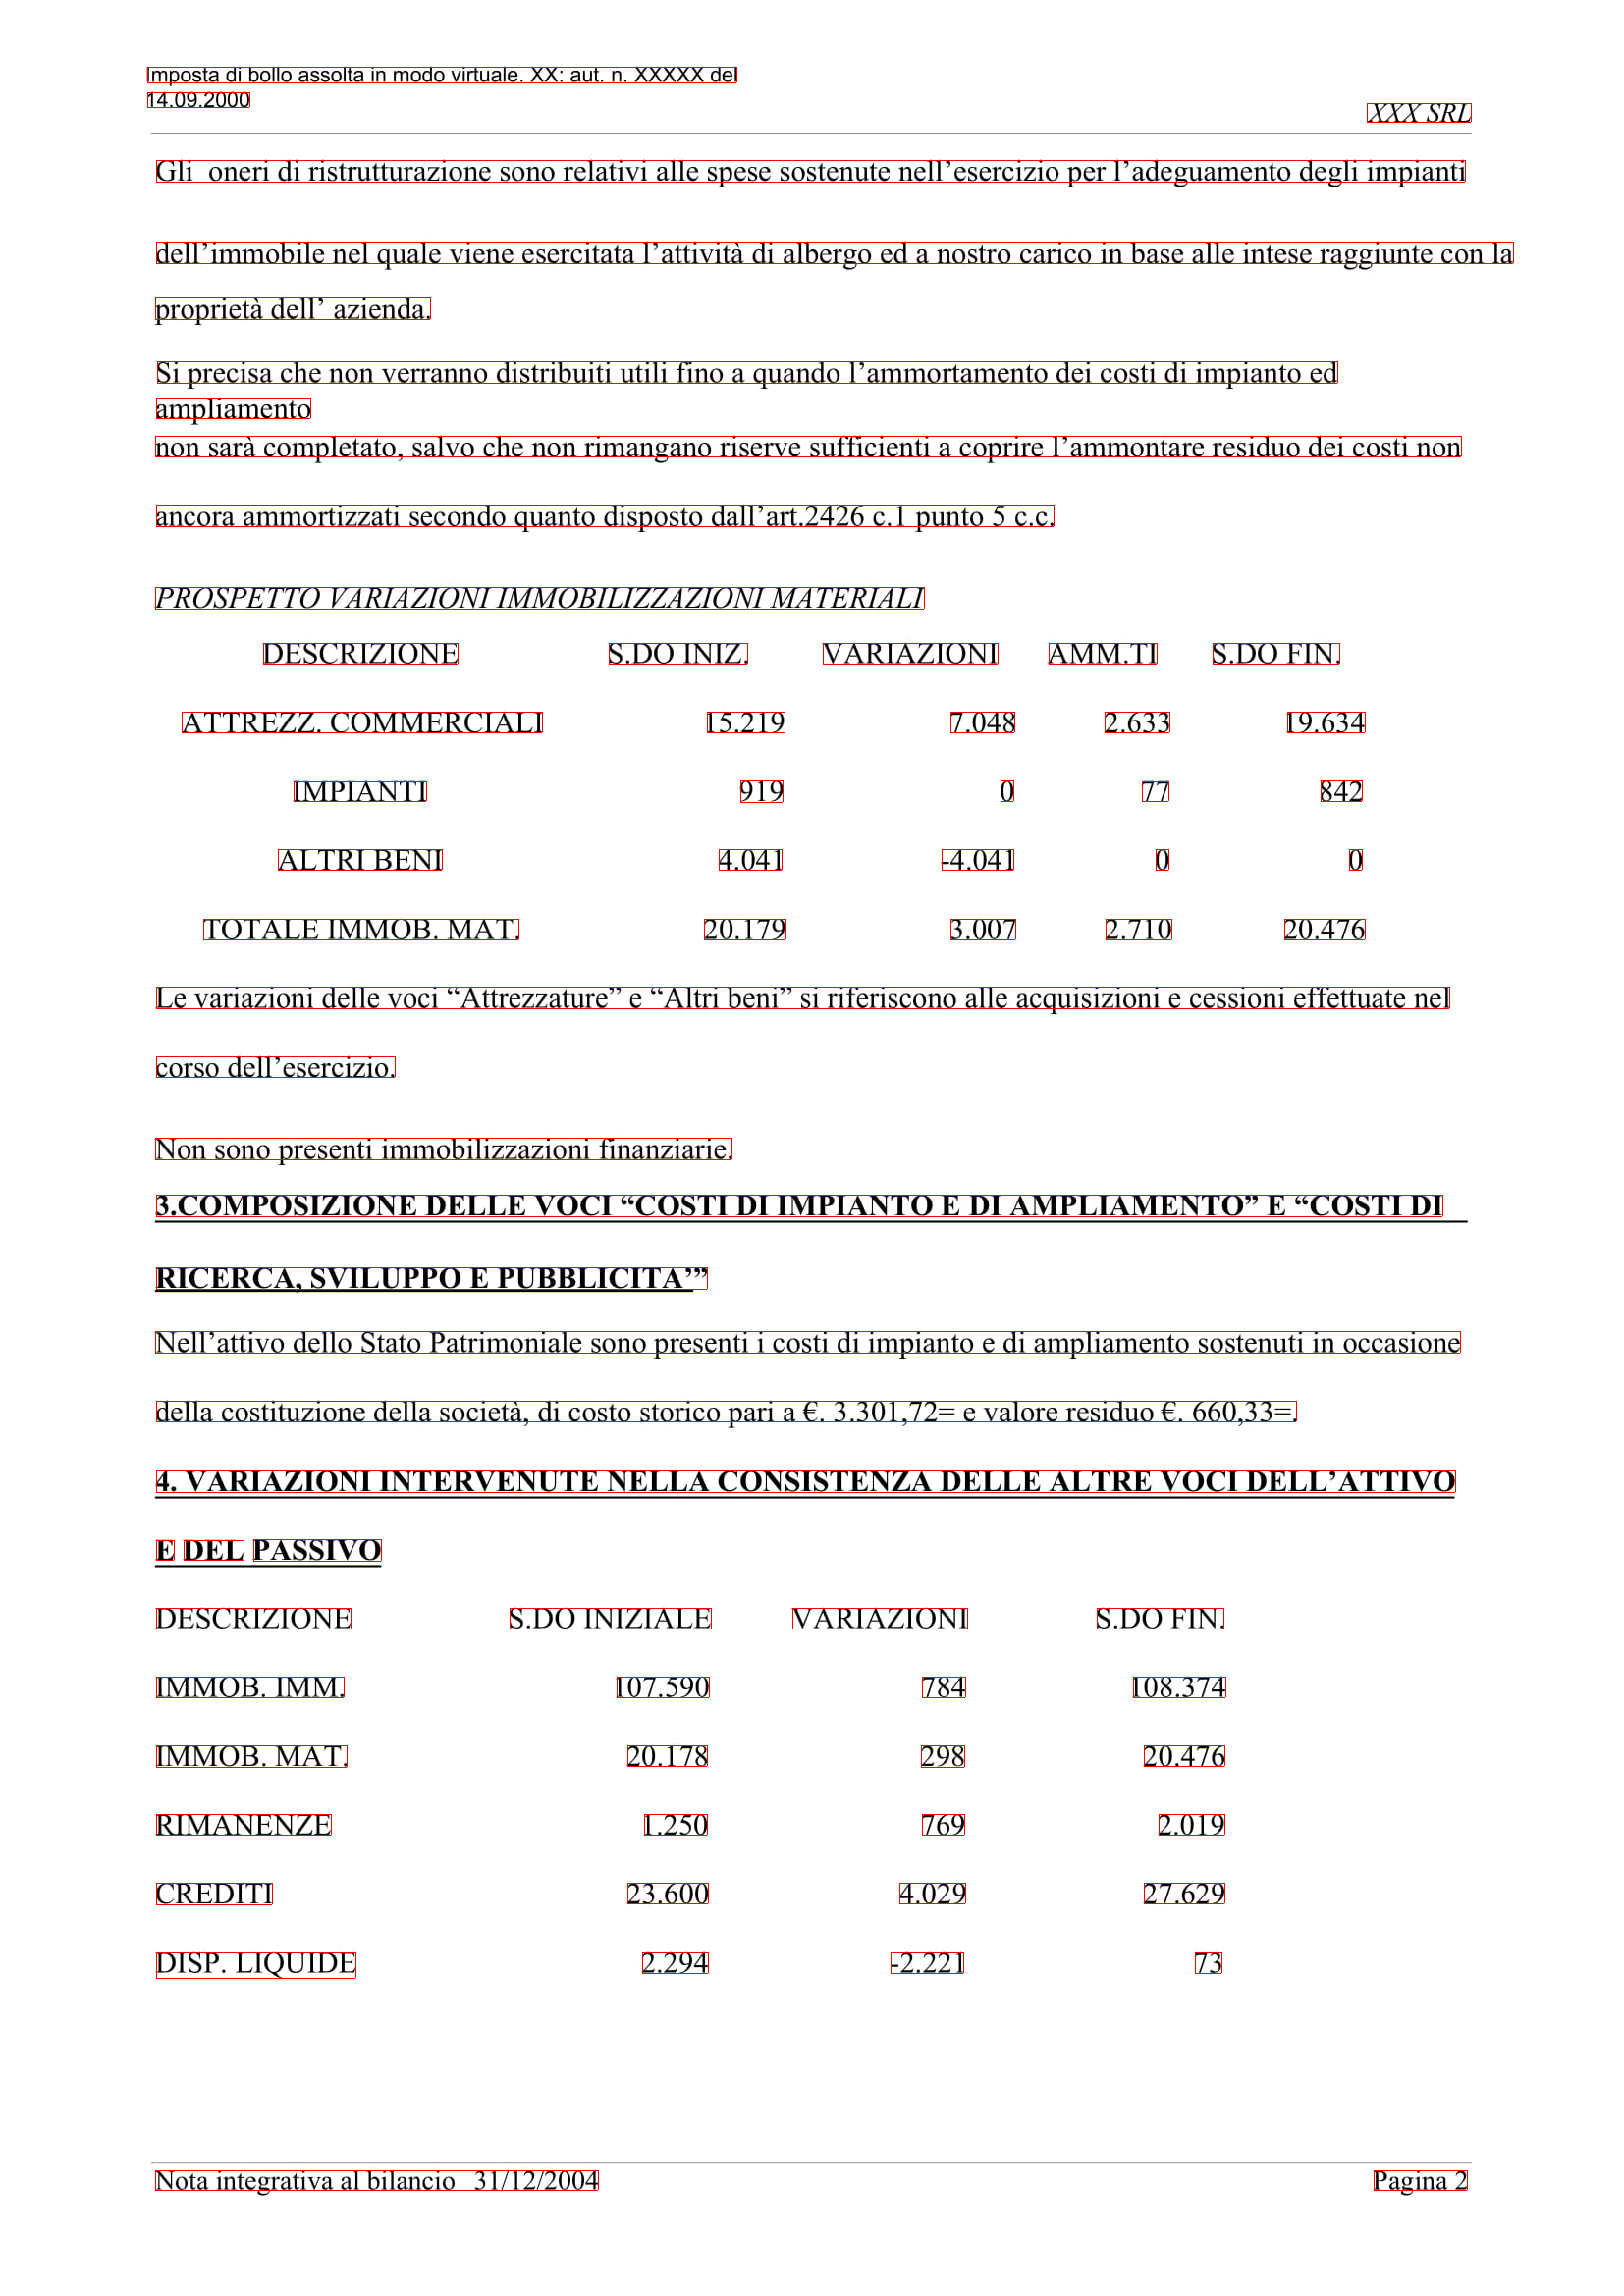
\includegraphics[width=\linewidth]{img/implementation/implem3.png}
\caption{Textlines merged into columns}
\label{fig:implem3}
\end{subfigure}
\qquad
\begin{subfigure}{0.45\textwidth}
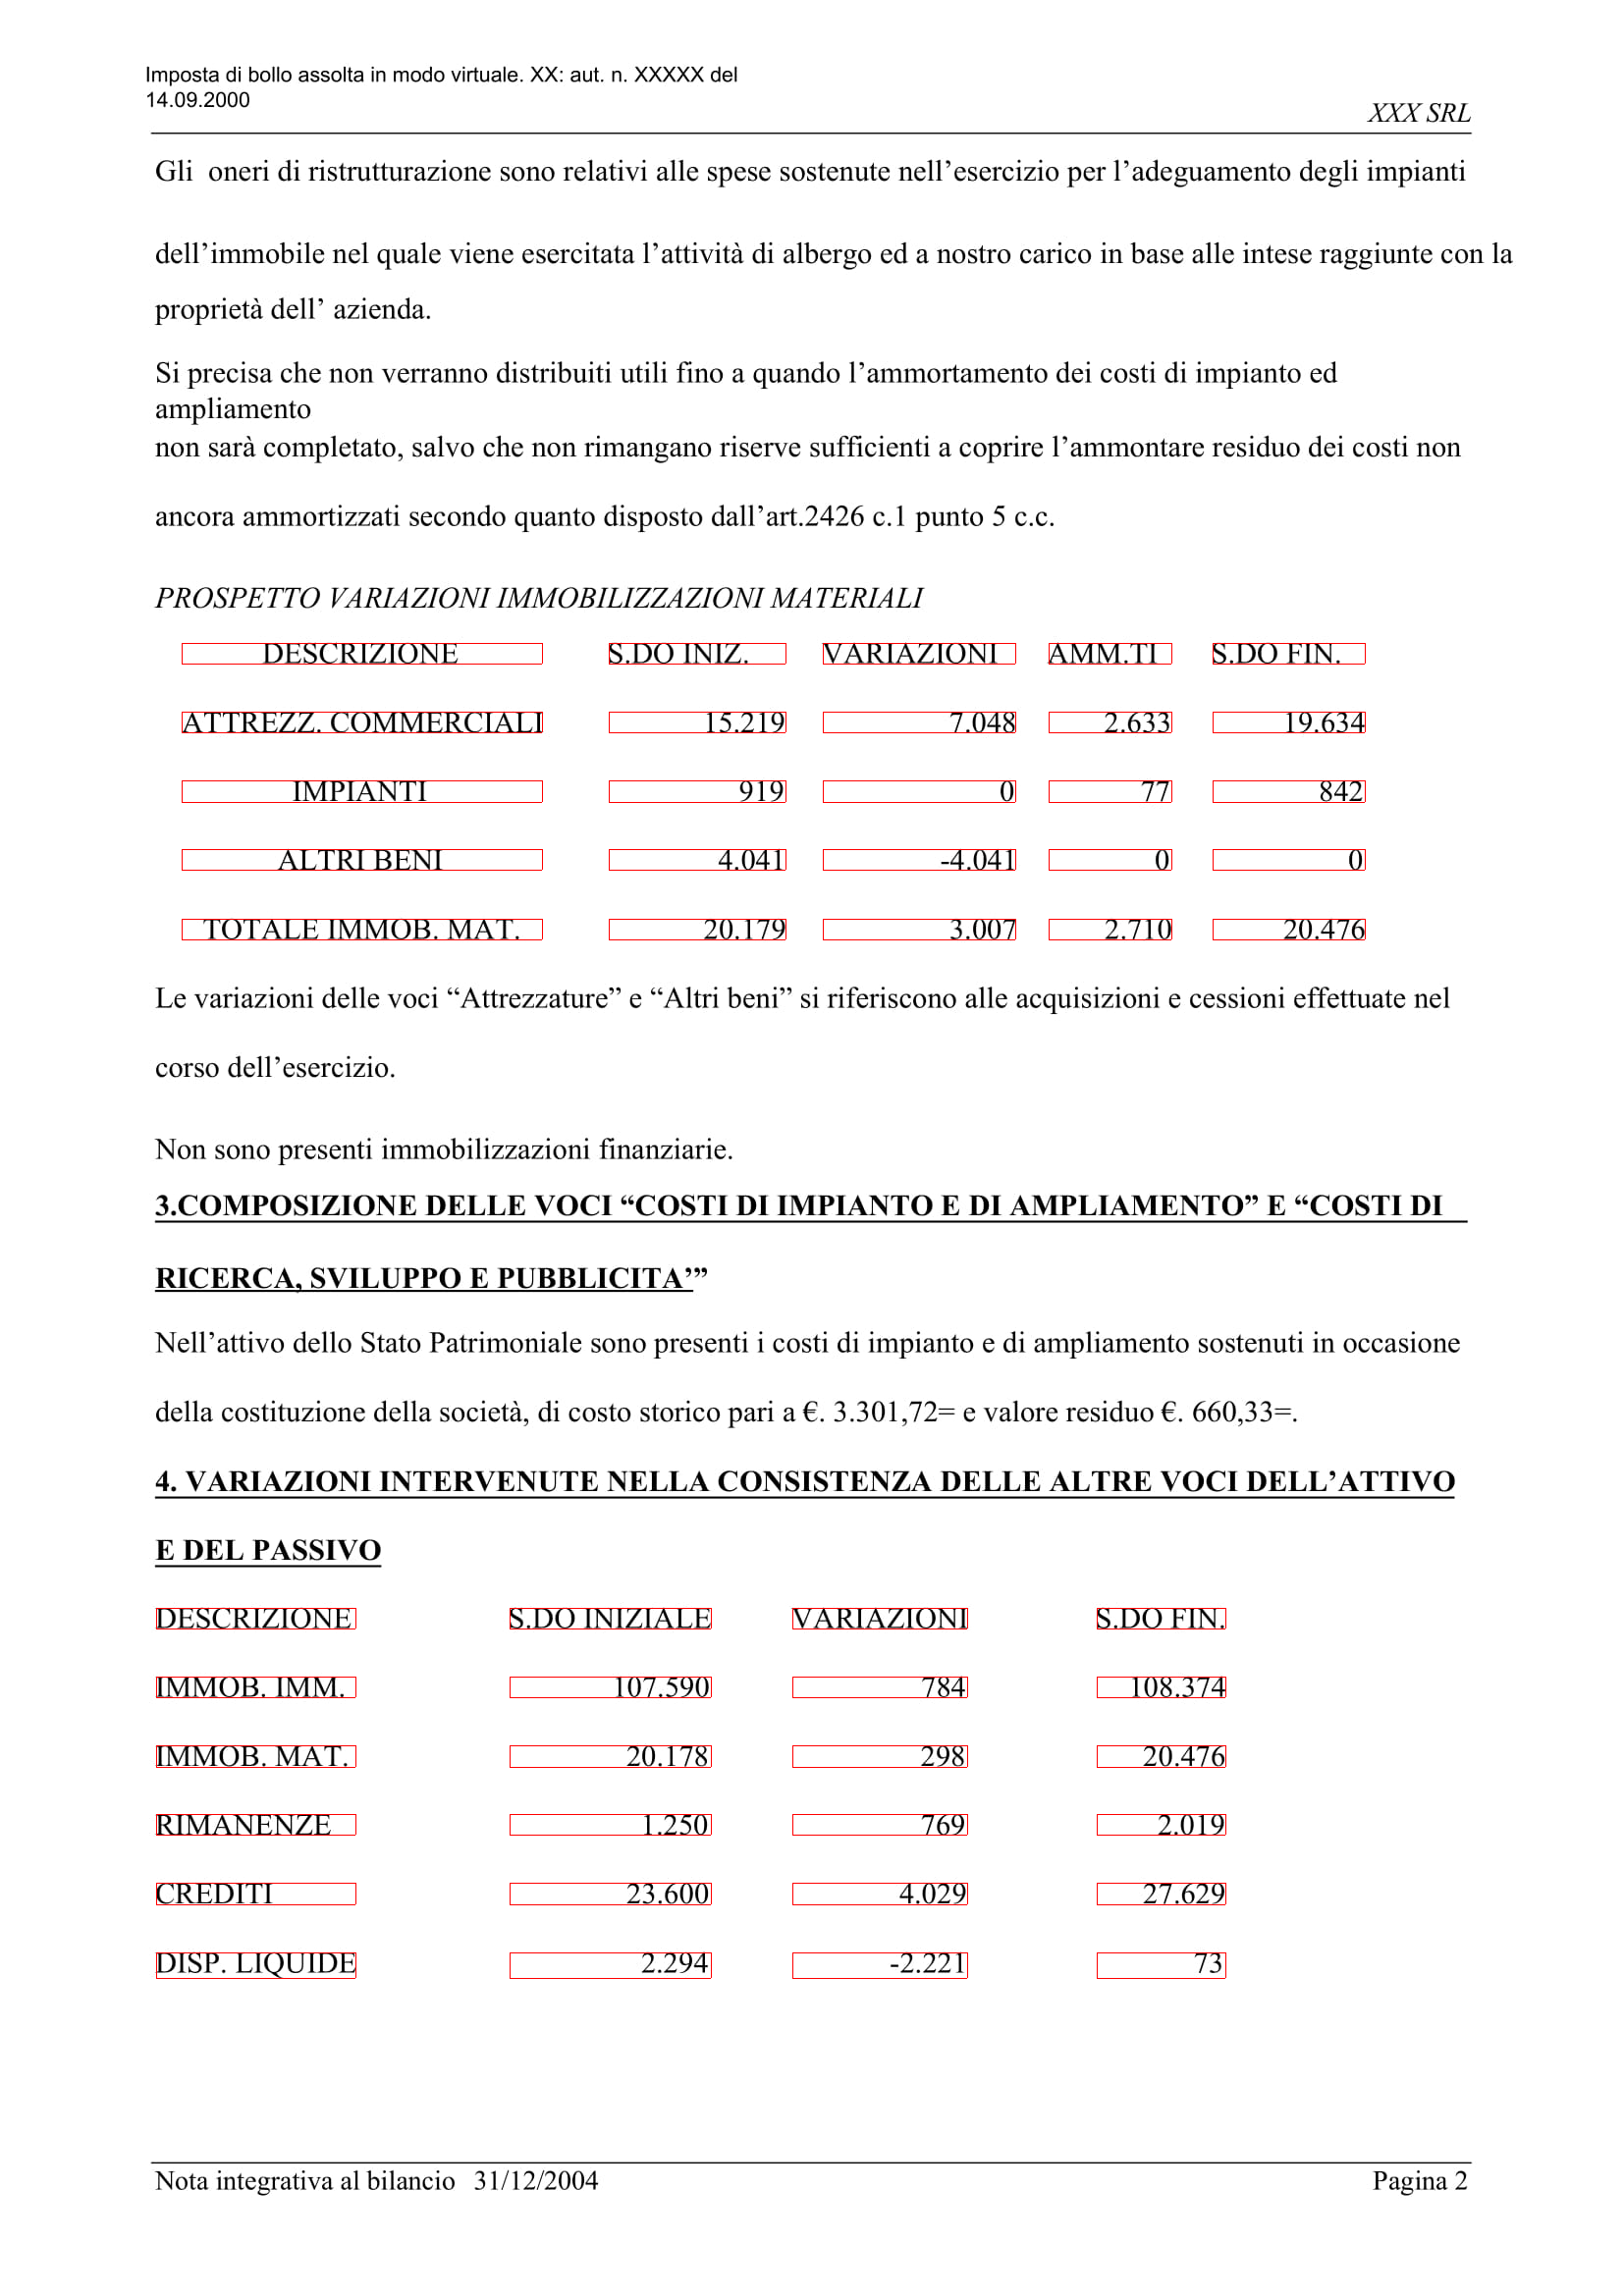
\includegraphics[width=\linewidth]{img/implementation/implem4.png}
\caption{The resulting cells}
\label{fig:implem4}
\end{subfigure}
\caption{The process of table recognition}
\label{fig:implemTableRecogniton}
\end{figure}

\begin{figure}[t]
    \centering
	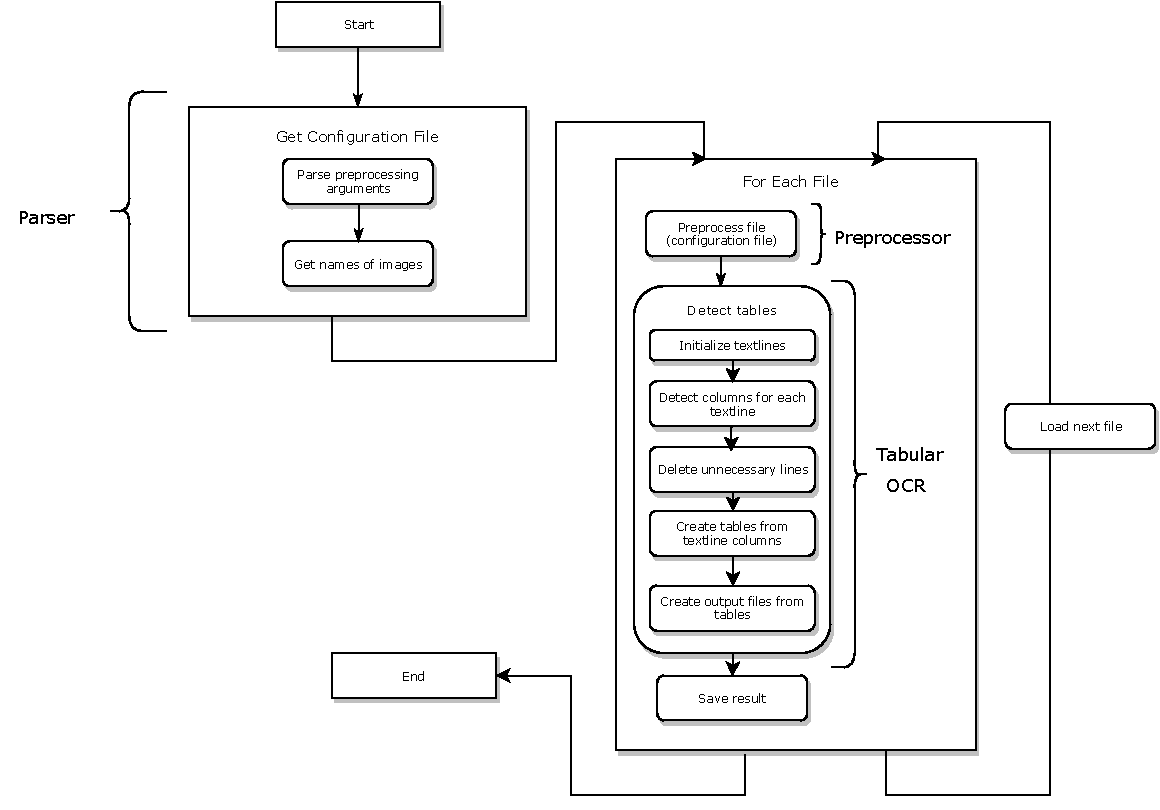
\includegraphics[width=1.0\linewidth]{img/implementation/programFlow.pdf}
	\caption{Program flow diagram}
	\label{fig:programFlow}
\end{figure}
